\documentclass[a4paper, 12pt]{article}
\usepackage[a4paper, top = 1.5cm, bottom = 1.5cm, left = 1cm, right = 1cm]{geometry}
\usepackage{graphicx}
\usepackage{subcaption}
\usepackage{mathtools}
\usepackage{amsfonts}
\usepackage[english, russian]{babel}
\title{Лабораторная работа № 3.5.1-3.5.2 "Изучение плазмы газового разряда в неоне"}
\author{Кирилл Шевцов Б03-402}
\date{16.09.2025}
\begin{document}
\maketitle
\section*{Цель работы}
Изучить вольт-амперную характеристику тлеющего разряда, изучить свойства плазмы методом зондовых
характеристик.
\section*{Оборудование}
Стеклянная газоразрядная трубка, наполненная неоном, источник напряжения, делитель напряжения, потенциометр,
амперметр, вольтметры, амперметры, переключатели.
\section*{Лабораторные установки}
Стеклянная газоразрядная трубка имеет ненагреваемый полый катод, три анода и геттерный узел - стеклянный баллон,
на внутреннюю поверхность которого напылена газопоглощающая плёнка (геттер). Трубка наполнена изотопом неона при давлении
2 мм. рт. столба. Катод и один из анодов (первый или второй) с помощью переключателя $P_{1}$ подключаются через балластный резистор
$R_{b}$ к регулируемому ВИП.
\begin{figure}[htbp]
    \centering
    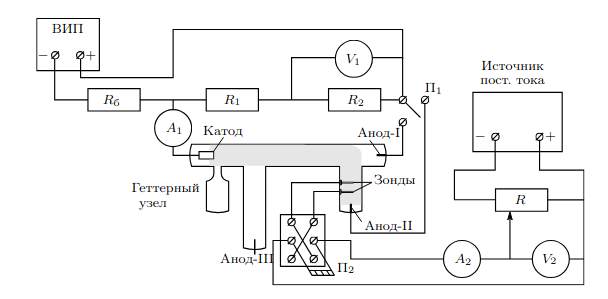
\includegraphics[width=0.6\linewidth]{p1.png}
    \caption{установка для исследования газового разряда}
    \label{установка для исследования газового разряда}
\end{figure}\\
При подключении первого анода к ВИП, между ним и катодом возникает газовый разряд. Ток разряда измеряется
амперметром $A_{1}$, падение напряжения - на вольтметре $V_{1}$, подключенным к трубке через делитель напряжения с
коэффициентом, равным $\alpha = \frac{R_{1} + R_{2}}{R_{2}}$. При подключении к ВИП второго анода, возникает газовый разряд между
катодами и вторым анодом, где находится двойной зонд, необходимый для диагностики плазмы. Третий анод в работе не используется.
\section*{Выполнение работы}
\end{document}